\documentclass[a4paper,landscape]{article}
%\usepackage[dutch]{babel}  % Removed - not available in this TeX distribution
\usepackage[utf8]{inputenc}
\usepackage{tikz}
\usepackage{hyperref}
\usepackage{geometry}
\usepackage{amsmath}
\usepackage{amssymb}
\usepackage{xcolor}

\geometry{margin=1cm}

\usetikzlibrary{shapes,arrows,positioning,calc,patterns,decorations.pathreplacing,decorations.markings,backgrounds,fit,shadows}

% Define colors
\definecolor{cecolor}{RGB}{220,50,50}        % Red for CE topics
\definecolor{secolor}{RGB}{50,120,200}       % Blue for SE-only topics
\definecolor{skillcolor}{RGB}{50,180,80}     % Green for skills
\definecolor{practicalcolor}{RGB}{255,200,50} % Yellow for practicals

\hypersetup{
    colorlinks=true,
    linkcolor=blue,
    urlcolor=blue,
    pdftitle={VMBO-TL Natuurkunde Routekaart GT3-GT4},
    pdfauthor={Natuurkunde Curriculum},
}

\pagestyle{empty}

\begin{document}

%==============================================================================
% TITLE PAGE
%==============================================================================
\begin{titlepage}
\centering
\vspace*{2cm}

{\Huge\bfseries VMBO-TL Natuurkunde\\[0.5cm] Interactieve Routekaart\\[0.5cm] GT3 \& GT4\par}

\vspace{1.5cm}

{\Large VMBO-TL - PTA Overzicht\par}

\vspace{2cm}

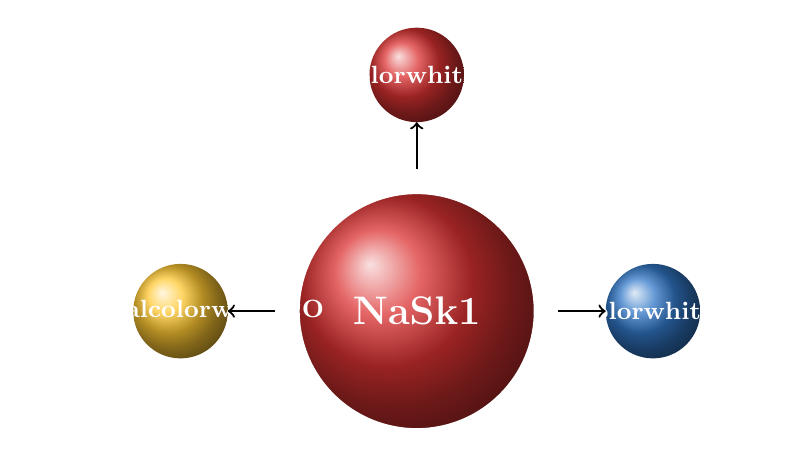
\begin{tikzpicture}[scale=1.5]
    % Central atom-like design
    \shade[ball color=cecolor] (0,0) circle (1cm);
    \draw[white,thick] (0,0) circle (1cm);
    \node[white,font=\Large\bfseries] at (0,0) {NaSk1};

    % Orbiting elements (removed V/Verdieping)
    \foreach \angle/\text/\color in {0/SE/secolor, 90/CE/cecolor, 180/PO/practicalcolor}{
        \shade[ball color=\color] (\angle:2) circle (0.4cm);
        \node[white,font=\small\bfseries] at (\angle:2) {\text};
        \draw[->,thick,\color] (\angle:1.2) -- (\angle:1.6);
    }
\end{tikzpicture}

\vspace{2cm}

{\large\itshape
Klik op elk vak in de routekaart\\
voor gedetailleerde uitleg\par}

\vfill

{\large Schooljaar 2025-2026\par}
{\normalsize Jaar 3: 100\% SE $\mid$ Jaar 4: Focus op CE $\mid$ Eindcijfer: 50\% SE + 50\% CE\par}

\end{titlepage}

%==============================================================================
% MAIN ROADMAP PAGE
%==============================================================================
\newpage

\section*{Natuurkunde Routekaart GT3 $\rightarrow$ GT4}

\vspace{0.5cm}

{\large\itshape\centering \textcolor{cecolor}{$\blacktriangleright$ Klik op elk vak voor details $\blacktriangleleft$}\par}

\vspace{0.5cm}

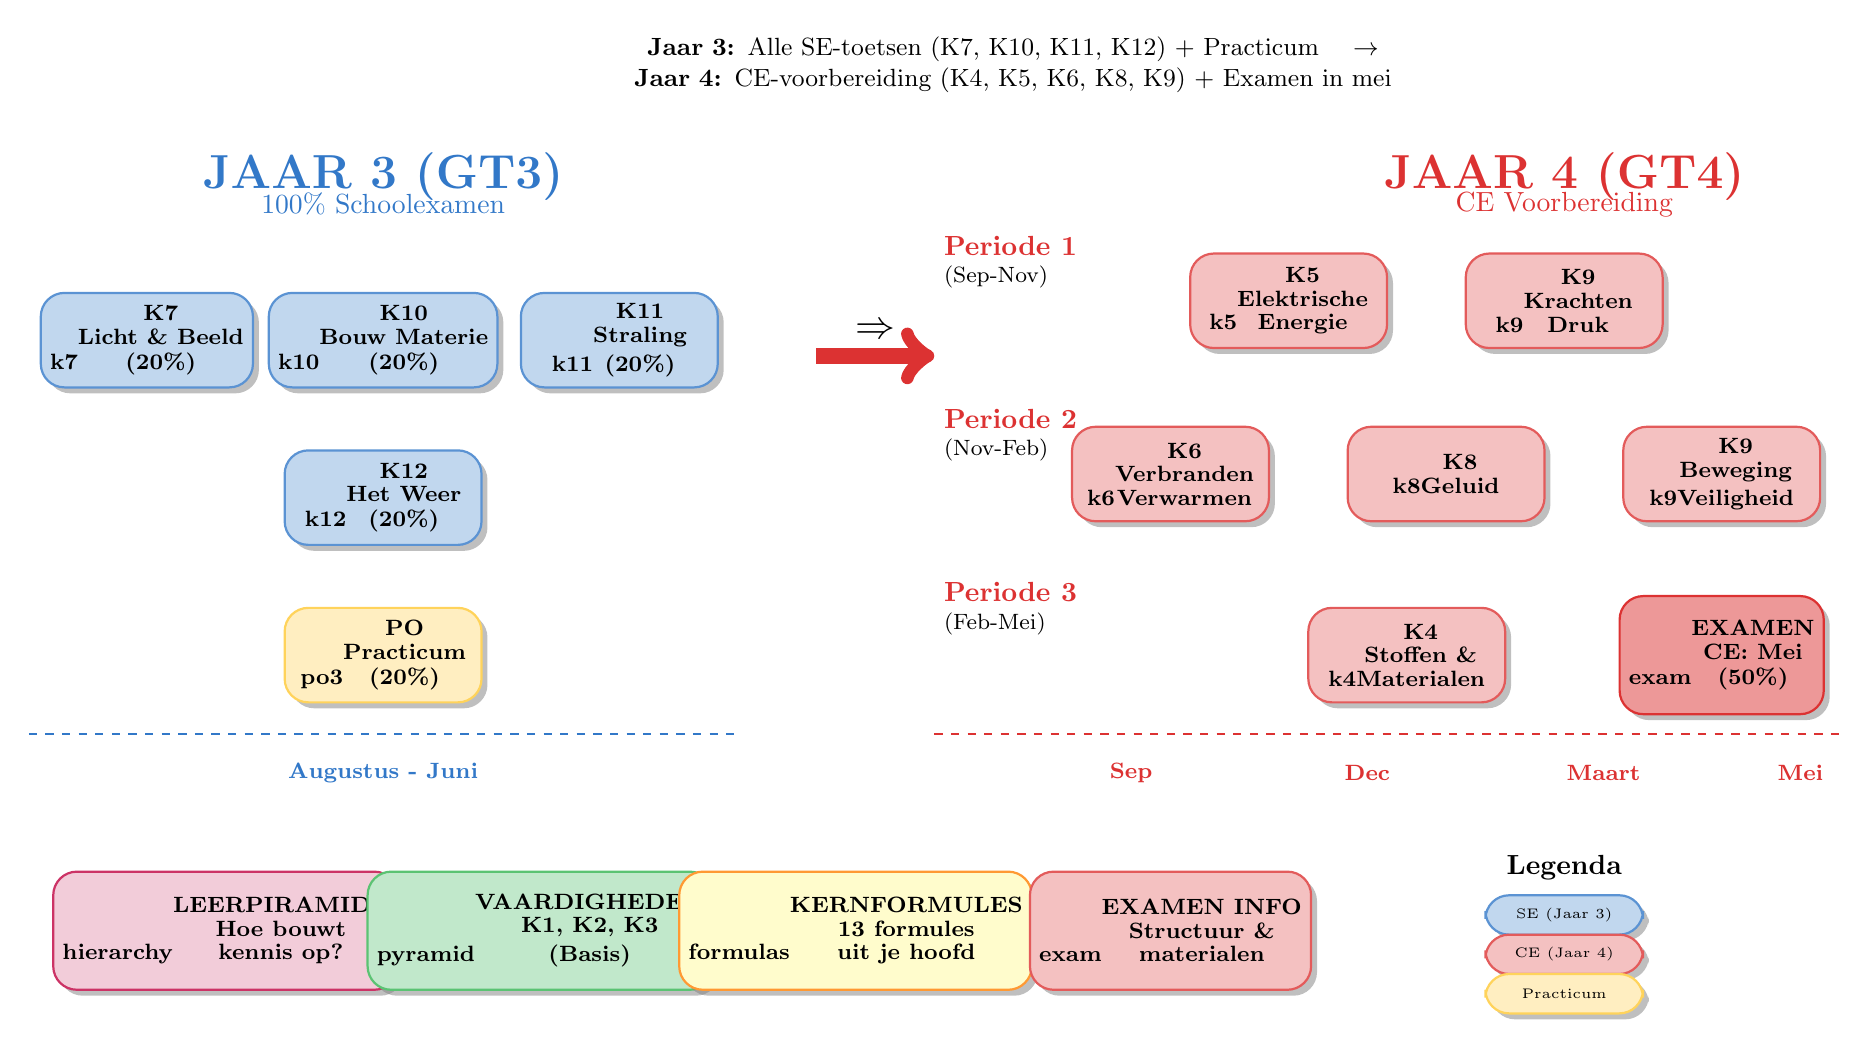
\begin{tikzpicture}[
    scale=1.0,
    every node/.style={font=\small},
    clickbox/.style={rectangle,rounded corners=3mm,draw,thick,minimum width=2.5cm,minimum height=1.2cm,align=center,drop shadow,font=\footnotesize\bfseries},
    cedomain/.style={clickbox,fill=cecolor!30,draw=cecolor!80},
    sedomain/.style={clickbox,fill=secolor!30,draw=secolor!80},
    skilldomain/.style={clickbox,fill=skillcolor!30,draw=skillcolor!80},
    practicaldomain/.style={clickbox,fill=practicalcolor!30,draw=practicalcolor!80},
]

%------------------------------------------------------------------------------
% INSTRUCTIONAL HEADER
%------------------------------------------------------------------------------
\node[font=\small,text width=18cm,align=center] at (0,7.5) {%
    \textbf{Jaar 3:} Alle SE-toetsen (K7, K10, K11, K12) + Practicum \quad $\rightarrow$ \quad
    \textbf{Jaar 4:} CE-voorbereiding (K4, K5, K6, K8, K9) + Examen in mei
};

%------------------------------------------------------------------------------
% YEAR 3 (GT3) - Left side
%------------------------------------------------------------------------------
\node[font=\LARGE\bfseries,secolor,anchor=north] at (-8,6.5) {JAAR 3 (GT3)};
\node[font=\normalsize,secolor,anchor=north] at (-8,6) {100\% Schoolexamen};

% SE domains - clickable
\node[sedomain] at (-11,4) {\hyperlink{k7}{\shortstack{\textbf{K7}\\Licht \& Beeld\\(20\%)}}};
\node[sedomain] at (-8,4) {\hyperlink{k10}{\shortstack{\textbf{K10}\\Bouw Materie\\(20\%)}}};
\node[sedomain] at (-5,4) {\hyperlink{k11}{\shortstack{\textbf{K11}\\Straling\\(20\%)}}};
\node[sedomain] at (-8,2) {\hyperlink{k12}{\shortstack{\textbf{K12}\\Het Weer\\(20\%)}}};
\node[practicaldomain] at (-8,0) {\hyperlink{po3}{\shortstack{\textbf{PO}\\Practicum\\(20\%)}}};

% Year 3 timeline
\draw[thick,secolor,dashed] (-12.5,-1) -- (-3.5,-1);
\node[font=\footnotesize\bfseries,secolor] at (-8,-1.5) {Augustus - Juni};

%------------------------------------------------------------------------------
% TRANSITION ARROW
%------------------------------------------------------------------------------
\draw[->,ultra thick,cecolor,line width=2mm] (-2.5,3.8) -- node[above,font=\Large\bfseries,black] {$\Rightarrow$} (-1,3.8);

%------------------------------------------------------------------------------
% YEAR 4 (GT4) - Right side
%------------------------------------------------------------------------------
\node[font=\LARGE\bfseries,cecolor,anchor=north] at (7,6.5) {JAAR 4 (GT4)};
\node[font=\normalsize,cecolor,anchor=north] at (7,6) {CE Voorbereiding};

% Period labels - moved left to prevent overlap with boxes
\node[font=\normalsize\bfseries,anchor=west,cecolor] at (-1,5.2) {Periode 1};
\node[font=\footnotesize,anchor=west] at (-1,4.8) {(Sep-Nov)};

\node[font=\normalsize\bfseries,anchor=west,cecolor] at (-1,3) {Periode 2};
\node[font=\footnotesize,anchor=west] at (-1,2.6) {(Nov-Feb)};

\node[font=\normalsize\bfseries,anchor=west,cecolor] at (-1,0.8) {Periode 3};
\node[font=\footnotesize,anchor=west] at (-1,0.4) {(Feb-Mei)};

% CE domains - clickable
% Period 1
\node[cedomain] at (3.5,4.5) {\hyperlink{k5}{\shortstack{\textbf{K5}\\Elektrische\\Energie}}};
\node[cedomain] at (7,4.5) {\hyperlink{k9}{\shortstack{\textbf{K9}\\Krachten\\Druk}}};

% Period 2
\node[cedomain] at (2,2.3) {\hyperlink{k6}{\shortstack{\textbf{K6}\\Verbranden\\Verwarmen}}};
\node[cedomain] at (5.5,2.3) {\hyperlink{k8}{\shortstack{\textbf{K8}\\Geluid}}};
\node[cedomain] at (9,2.3) {\hyperlink{k9}{\shortstack{\textbf{K9}\\Beweging\\Veiligheid}}};

% Period 3
\node[cedomain] at (5,0) {\hyperlink{k4}{\shortstack{\textbf{K4}\\Stoffen \&\\Materialen}}};

% Exam
\node[cedomain,minimum height=1.5cm,fill=cecolor!50,draw=cecolor] at (9,0) {%
    \hyperlink{exam}{\shortstack{\textbf{EXAMEN}\\CE: Mei\\(50\%)}}};

% Year 4 timeline - aligned with period labels
\draw[thick,cecolor,dashed] (-1,-1) -- (10.5,-1);
\node[font=\footnotesize\bfseries,cecolor] at (1.5,-1.5) {Sep};
\node[font=\footnotesize\bfseries,cecolor] at (4.5,-1.5) {Dec};
\node[font=\footnotesize\bfseries,cecolor] at (7.5,-1.5) {Maart};
\node[font=\footnotesize\bfseries,cecolor] at (10,-1.5) {Mei};

%------------------------------------------------------------------------------
% BOTTOM SECTION: Skills, Formulas, Legend
%------------------------------------------------------------------------------

% Learning hierarchy - NEW!
\node[clickbox,fill=purple!20,draw=purple!80,minimum width=3cm,minimum height=1.5cm] at (-10,-3.5) {%
    \hyperlink{hierarchy}{\shortstack{\textbf{LEERPIRAMIDE}\\Hoe bouwt\\kennis op?}}};

% Skills pyramid - clickable
\node[skilldomain,minimum width=3cm,minimum height=1.5cm] at (-6,-3.5) {%
    \hyperlink{pyramid}{\shortstack{\textbf{VAARDIGHEDEN}\\K1, K2, K3\\(Basis)}}};

% Formulas - clickable
\node[clickbox,fill=yellow!20,draw=orange!80,minimum width=3cm,minimum height=1.5cm] at (-2,-3.5) {%
    \hyperlink{formulas}{\shortstack{\textbf{KERNFORMULES}\\13 formules\\uit je hoofd}}};

% Exam info - clickable
\node[cedomain,minimum width=3cm,minimum height=1.5cm] at (2,-3.5) {%
    \hyperlink{exam}{\shortstack{\textbf{EXAMEN INFO}\\Structuur \&\\materialen}}};

% Legend
\begin{scope}[shift={(7,-3.5)}]
    \node[font=\normalsize\bfseries] at (0,0.8) {Legenda};
    \node[sedomain,minimum width=2cm,minimum height=0.5cm,font=\tiny] at (0,0.2) {SE (Jaar 3)};
    \node[cedomain,minimum width=2cm,minimum height=0.5cm,font=\tiny] at (0,-0.3) {CE (Jaar 4)};
    \node[practicaldomain,minimum width=2cm,minimum height=0.5cm,font=\tiny] at (0,-0.8) {Practicum};
\end{scope}

\end{tikzpicture}

\newpage

%==============================================================================
% INCLUDED SECTIONS
%==============================================================================

% Learning hierarchy - shows how knowledge builds
\input{sections/learning_hierarchy.tex}

% Skills domains (K1, K2, K3)
\input{sections/skills.tex}

% Year 3 SE-only domains (K7, K10, K11, K12)
\input{sections/year3_domains.tex}

% Year 4 CE domains (K4, K5, K6, K8, K9)
\input{sections/year4_domains.tex}

% Centraal Examen information
\input{sections/exam.tex}

% Formulas reference
\input{sections/formulas.tex}

\end{document}
